\section{Curvature-induced effects in flat magnetic systems}\label{sec:curvature_effects}

The purpose of this section is to demonstrate that curvature of the ferromagnetic (FM) wire is a source of new equilibrium states and it also influences the spin-wave dynamics. We will consider equilibrium states and linear dynamics of the magnetization in wires with constant, box-function, and periodic curvature distributions.

Within this section, it is convenient to introduce angular parametrization of the magnetization in the local Frenet--Serret reference of frame as follows $\vec{m} =\sin\theta\,\left(\cos\phi\,\vec{e}_\textsc{t} + \sin\phi\,\vec{e}_\textsc{n}\right) + \cos\theta\,\vec{e}_\textsc{b}$, where $\theta=\theta(\overline{t},\xi)$ and $\phi=\phi(\overline{t},\xi)$ are magnetic angles. With this angular notations, one can rewrite the equations of motion~\eqref{eq:llg} as
\begin{equation}\label{eq:llg_angular}
\sin\theta\, \dot{\phi} = \frac{\delta \mathcal{E}}{\delta \theta}+\alpha_\textsc{g} \dot{\theta},\quad -\sin\theta\,\dot{\theta} = \frac{\delta \mathcal{E}}{\delta \phi}+\alpha_\textsc{g}\sin^2\theta\, \dot{\phi}
\end{equation}
with energy in angular parametrization
\begin{equation}\label{eq:energy_angular}
\begin{split}
\mathcal{E} = \int\mathrm{d}\xi\bigl[\left(\theta'\right)^2+\sin^2\theta\,\left(\phi'+\varkappa\right)^2-\sin^2\theta\cos^2\phi\bigr].
\end{split}
\end{equation}
In \eqref{eq:energy_angular} it is taken into account that a plane wires have zero torsion.

\subsection{Wire with a constant curvature -- ring shaped wire}\label{sec:rings}

Here, we consider a flat anisotropic FM nanowire with a fixed cross-section of area $S$ and constant curvature -- ring shaped wire, see Fig.~\ref{fig:Geometries_n_curvatures}(a). The ring geometry is a prototypical example of a highly-symmetrical curved system with constant curvature $\varkappa=\text{const}$. It was investigated intensively both experimentally~\cite{Klaui01,Klaui03a,Klaui05a} and theoretically~\cite{Kravchuk09,Kravchuk11,Sheka15}.% due to the potential applications in magnetic storage media. To control the recording element it is necessary to have at least two different equilibrium magnetization states and well defined switching mechanism between them. In the case of magnetic nanorings made from soft magnetic materials the main equilibrium state is a \textit{vortex state} in which the magnetic flux is closed in the element.

\subsubsection{Equilibrium states}\label{sec:rings_equilibrium}

For the case ring-shaped nanowire with constant curvature, the minimization of energy~\eqref{eq:energy_angular} results in the solution $\theta_0=\pi/2$ and the azimuthal angle $\phi$, which
satisfies the pendulum equation
\begin{equation}\label{eq:ring_phi}
\phi'' - \sin\phi\cos\phi = 0.
\end{equation}
This equation has a trivial solution in curvilinear reference of frame which correspond to the \textit{vortex} magnetization distribution with
\begin{equation}\label{eq:ring_vortex}
\theta_0^\text{vor}=\pi/2,\quad \cos\phi_0^\text{vor} = \mathcal{C}=\pm 1,
\end{equation}
which is well known for the magnetic nanorings. Parameter $\mathcal{C}=\pm1$ is a chirality of the magnetization distribution, i.e $\mathcal{C}=+1$ and $\mathcal{C}=-1$ correspond to the clockwise and counterclockwise magnetization distribution, respectively. This state is typical for relatively large rings (rings with small curvature) and describes flux-free magnetization distribution, see Fig.~\ref{fig:ring_states}(a).

%==================================================================\
\begin{figure}[t]
	\centering
	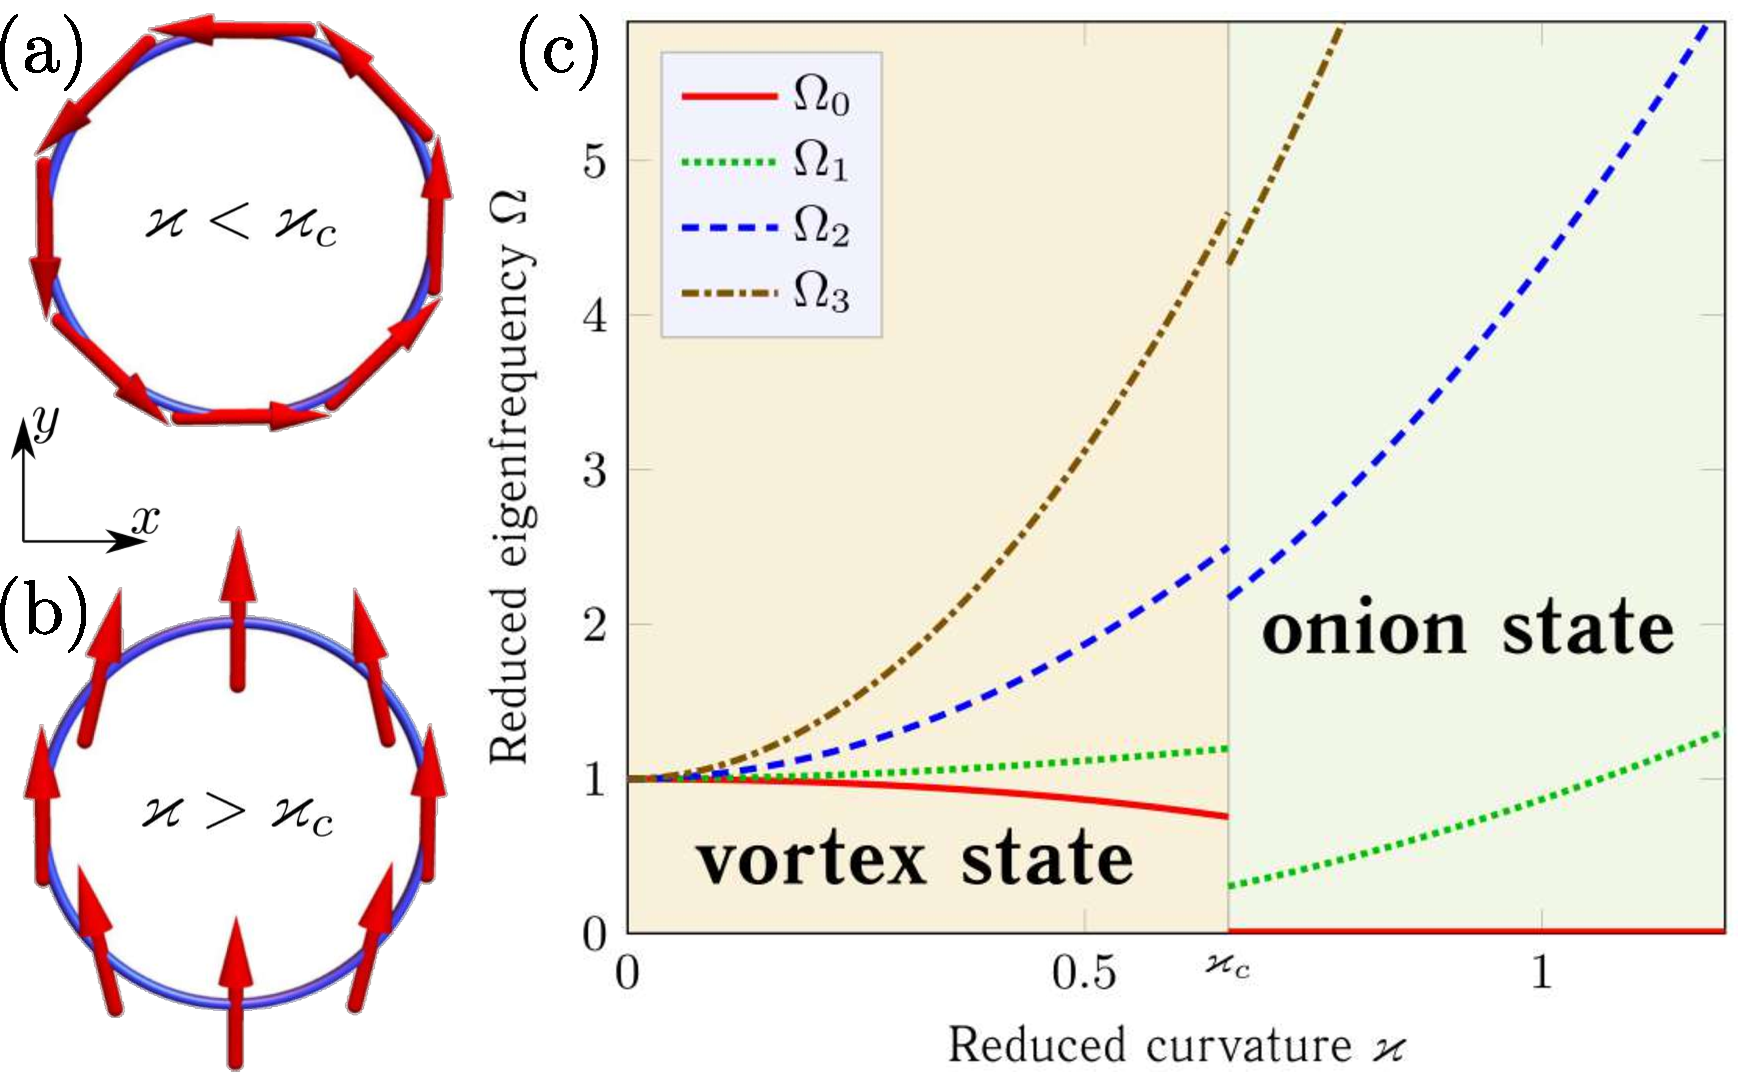
\includegraphics[width=0.8\textwidth]{fig_ring_states}
	\caption{\label{fig:ring_states}%
		\textbf{Nanoring wire:} Magnetization distribution of the ground state in a ring wire with different reduced curvatures: (a) vortex state for $\varkappa<\varkappa_c$ and (b) onion state for $\varkappa>\varkappa_c$. (c) The lowest eigenfrequencies of linear excitations in a ring nanowire depending on the curvature $\varkappa$. Adapted with permission from~\cite{Sheka15}.}
\end{figure}
%==================================================================/

Equation~\eqref{eq:ring_phi} also has an inhomogeneous solution in curvilinear reference of frame
\begin{equation}\label{eq:ring_onion}
\theta_0^\text{on}=\pi/2,\quad \phi_0^\text{on}(\xi)=\text{am}\left[\xi/k,k\right].
\end{equation}
where $\text{am}\left(x,y\right)$ is the Jacobi amplitude~\cite{NIST10} and the modulus $k$ is determined by the condition $2\varkappa k \mathrm{K}(k)=\pi$ with $\mathrm{K}(k)$ being the complete elliptic integral of the first kind~\cite{NIST10}. This state is characterized with a quasi-uniform magnetization distribution in Cartesian reference of frame, see Fig.~\ref{fig:ring_states}(b). This state is an arrangement of magnetic moments in which the ring is divided into two magnetic domains separated by two domain walls, with magnetization oriented tangentially in two different directions, clockwise and counterclockwise. This structure is usually referred to as an \textit{onion} state~\cite{Klaui03a}.  One should note that for the case of magnetoelastic rings, the onion state~\eqref{eq:ring_onion} results in deformation of the ring shape from circular to the elliptic-like geometry~\cite{Gaididei19}.

Both \textit{vortex} and \textit{onion} equilibrium states correspond to the planar magnetization distribution within the wire plane.

Nanorings with \textit{vortex} magnetization ground state can be prepared with smaller radii than nanodisks with the same magnetization structure~\cite{Kravchuk07}. The critical radius which separates the \textit{vortex} and \textit{onion} states defined, in general, by the relation $\varkappa_c \approx 0.657$~\cite{Sheka15}. For the permalloy nanoring we have  critical radius $R_{c}\approx 17$ nm, i.e. for rings with $R>R_c$ one obtains \textit{vortex} state, while for $R<R_c$ -- \textit{onion} state.

%As it was mentioned above, two domains in the \textit{onion} state are separated by two domain walls. Depending on the width of the ring one can obtain a transverse head-to-head~(tail-to-tail) DWs for narrow ribbons, or vortex head-to-head~(tail-to-tail) domain walls for wide rings, see Fig.~\ref{fig:ring_states}.

\subsubsection{Magnon spectrum in the ferromagnetic ring}\label{sec:ring_eigenmodes}

In the Sec.~\ref{sec:theory_1D} it is shown that nontrivial geometry results in appearance of the effective exchange-driven DMI and anisotropy. Therefore, one should expect the modification of magnon spectrum similar to the systems with an intrinsic DMI. To analyse the magnons in the curved system, we linearize the LLG equation~\eqref{eq:llg_angular} for zero damping $\alpha_\textsc{g}=0$ on the background of the vortex~\eqref{eq:ring_vortex} and onion~\eqref{eq:ring_onion} states with the substitution $\theta=\theta_0+\vartheta(\overline{t},\xi)$ and $\phi=\phi_0+\varphi(\overline{t},\xi)$. The linearizaed equations of motion reads as~\cite{Sheka15,Gaididei18a,Korniienko19b}
\begin{equation}\label{eq:ring_magnons}
-\vartheta''+V_1\vartheta = \dot{\varphi},\quad  -\varphi''+V_2\varphi = -\dot{\vartheta},
\end{equation}
where $V_1 = \cos^2\phi_0 - \left[\phi_0'+\varkappa(\xi)\right]^2$ and $V_2 = \cos2\phi_0$ are geometry-induced potentials.

For the simplest case of the ring-shaped wire with constant curvature $\varkappa=\text{const}$ and \textit{vortex} magnetization distribution one obtain $V_1=1-\varkappa^2$ and $V_2=1$. The set~\eqref{eq:ring_magnons} can be solved with plane waves ansatz $\vartheta=\sum_j \vartheta_j \cos(j\xi\varkappa-\Omega\overline{t}+\delta_j)$ and $\varphi=\sum_j \varphi_j \sin(j\xi\varkappa-\Omega\overline{t}+\delta_j)$ with $j$ being the azimuthal quantum number, $\delta_j$ is an arbitrary phase, and $\Omega$ is dimensionless frequency measured in units $\omega_0$. By substituting this ansatz in the set~\eqref{eq:ring_magnons} we can calculate the spectrum of magnon eigenstates as
\begin{equation}\label{eq:spec_rings}
\Omega^\text{vor}_j = \sqrt{\left(V_1+j^2\varkappa^2\right)\left(V_2+j^2\varkappa^2\right)}.
\end{equation}
The corresponding lower eigenfrequencies are plotted in the Fig.~~\ref{fig:ring_states}(c). For the limit case of the small curvature $\varkappa\ll1$~(quasi-straight wire), the magnon frequencies read
\begin{equation}\label{eq:spec_rings_small}
\Omega^\text{vor}_j = 1- \frac{\varkappa^2}{2}+j^2\varkappa^2+\mathcal{O}(\varkappa^4).
\end{equation}
Thus the curvature decreases the gap as compared to the case of the straight wire~($\varkappa=0$) with dispersion $\Omega^\text{str} = 1 + \mathfrak{K}^2$, where $\mathfrak{K}=j\varkappa$ is the corresponding normalized wave vector.

For the case of the \textit{onion} magnetization distribution \eqref{eq:ring_onion} the corresponding lower eigenfrequencies can be estimated as~\cite{Sheka15}
\begin{equation}\label{eq:spec_rings_onion}
	\Omega^\text{on}_j = \sqrt{\left(\mathcal{V}_1+j^2\varkappa^2\right)\left(\mathcal{V}_2+j^2\varkappa^2\right)},
\end{equation}
where $\mathcal{V}_1 = 1/k^2 + \varkappa^2 - 4\varkappa\mathrm{E}(k) /\left(k\pi\right)$ and  $\mathcal{V}_2 = 2/k^2 - 1 - 4\varkappa\mathrm{E}(k) /\left(k\pi\right)$ are first terms in the Fourier expansions of potential $V_1$ and $V_2$, respectively. Here, $\mathrm{E}(k)$ is the complete elliptic integral of the second kind~\cite{NIST10}. The corresponding lower eigenfrequencies are plotted in the Fig.~\ref{fig:ring_states}(c). Equation~\eqref{eq:spec_rings_onion} does not take into account the modes coupling, which can lead in the mixing of different partial waves.

The limit case $\Omega^\text{on}_0 = 0$ corresponds to the zero (Goldstone) mode, which is realized due to the arbitrary direction of the onion axis. Here, Goldstone mode contains an infinite number of partial waves; hence the coupling between different partial waves for this mode is crucial~\cite{Sheka15}.

\subsection{Wire with a box-function curvature} \label{sec:box_curvature}

%Wide variety of linear and non-linear spin-wave phenomena attracted the interest into the fundamental properties of the spin waves~\cite{Holstein40,Dyson56,Akhiezer68}, whereas their transport abilities are of the great interest for spintronics logical and signal-carrying elements~\cite{Khitun08,Schneider08,Khi10jpd,Vogt12}. Due to the possibility of building compact and low-power logical devices, spin waves are considered as potential data carriers for novel computing devices~\cite{Kruglyak10a,Lenk11,Chumak14,Chumak15,Mahmoud20}. However, in order to exploit spin waves for data processing in real devices, it requires unimpeded spin waves propagation in flat curvilinear structures with complicated geometry. This obliges the use of magnetic waveguides with ring segments of different sizes to preserve save space on chips~\cite{Vogt12,Xing13,Haldar16}, see Fig.~\ref{fig:Circular_segment_1}(a).

Here, we consider a flat anisotropic FM nanowire with a fixed cross-section of area $S$ and localized box-function curvature profile: $\varkappa (\xi) = \varkappa_0 \, \mathrm{H}(\xi+\xi_0) - \varkappa_0 \, \mathrm{H}(\xi-\xi_0)$, see Fig.~\ref{fig:Geometries_n_curvatures}(b).  Here, $\mathrm{H}(x)$ is the Heaviside step function, $\varkappa_0=\ell/R$ is the curvature of the arc bending with $R$ being the ring segment radius, and $\xi_0\varkappa_0 = (\pi-\alpha)/2$ with $\alpha$ being the expansion angle, see Fig.~\ref{fig:Circular_segment_1}.

\subsubsection{Equilibrium state} \label{sec:box_curvature_equilibrium}

%Based on Eq.~\ref{eq:Exchange_energy_TNB_2} and general theoretical approach introduced in \ref{sec:model_1D}, let us consider a flat anisotropic ferromagnetic nanowire with a fixed cross-section of area $S$ and localized box-function curvature profile: $\kappa (s) = \kappa_0 \, h(s+s_0) - \kappa_0 \, h(s-s_0)$, see Fig.~\ref{fig:Circular_segment_1}(b) and (c). Here, $h(\xi)$ is the Heaviside step function, $\kappa_0=1/R$ is the curvature of the arc bending with $R$ being the ring segment radius, and $\xi_0 = (\pi-\alpha)R/(2{\ell})$ with $\alpha$ being the expansion angle. To simplify the analytical consideration it is convenient to introduce the angular parameterization of the magnetization in the Frenet-Serret local reference frame, $\vec{m} = \sin\theta \, \cos\phi \, \vec{e}_{\textrm{T}}+\sin\theta \, \sin\phi \, \vec{e}_{\textrm{T}} + \cos\theta \, \vec{e}_{\textrm{B}}$, where the angular variables $\theta $ and $\phi $ depend on spacial and temporal coordinates. In the curvilinear reference frame the total energy \eqref{eq:total_energy} reads 

%\begin{equation} \label{eq:Energy-plane}
%E = S \, K_\text{eff} \, \int\mathrm{d}\vec{s}\, \left[ \ell^2 \, {\theta'}^2 + \ell^2 \, \sin^2\theta \, \left(\phi'+\kappa\right)^2 - \sin^2\theta\,\cos^2\phi \right],
%\end{equation}
%where $\ell=\sqrt{\mathcal{A}/K_\text{eff}}$ is the characteristic magnetic length, with $K_\text{eff}=K+\pi M_s^2$ being the constant of the effective easy-tangential anisotropy, that consists of the intrinsic crystalline anisotropy $K$ and the shape-induced magnetostatic contribution~\cite{Gaididei17a}. 

%==================================================================\
\begin{figure}[b]
	\begin{center}
		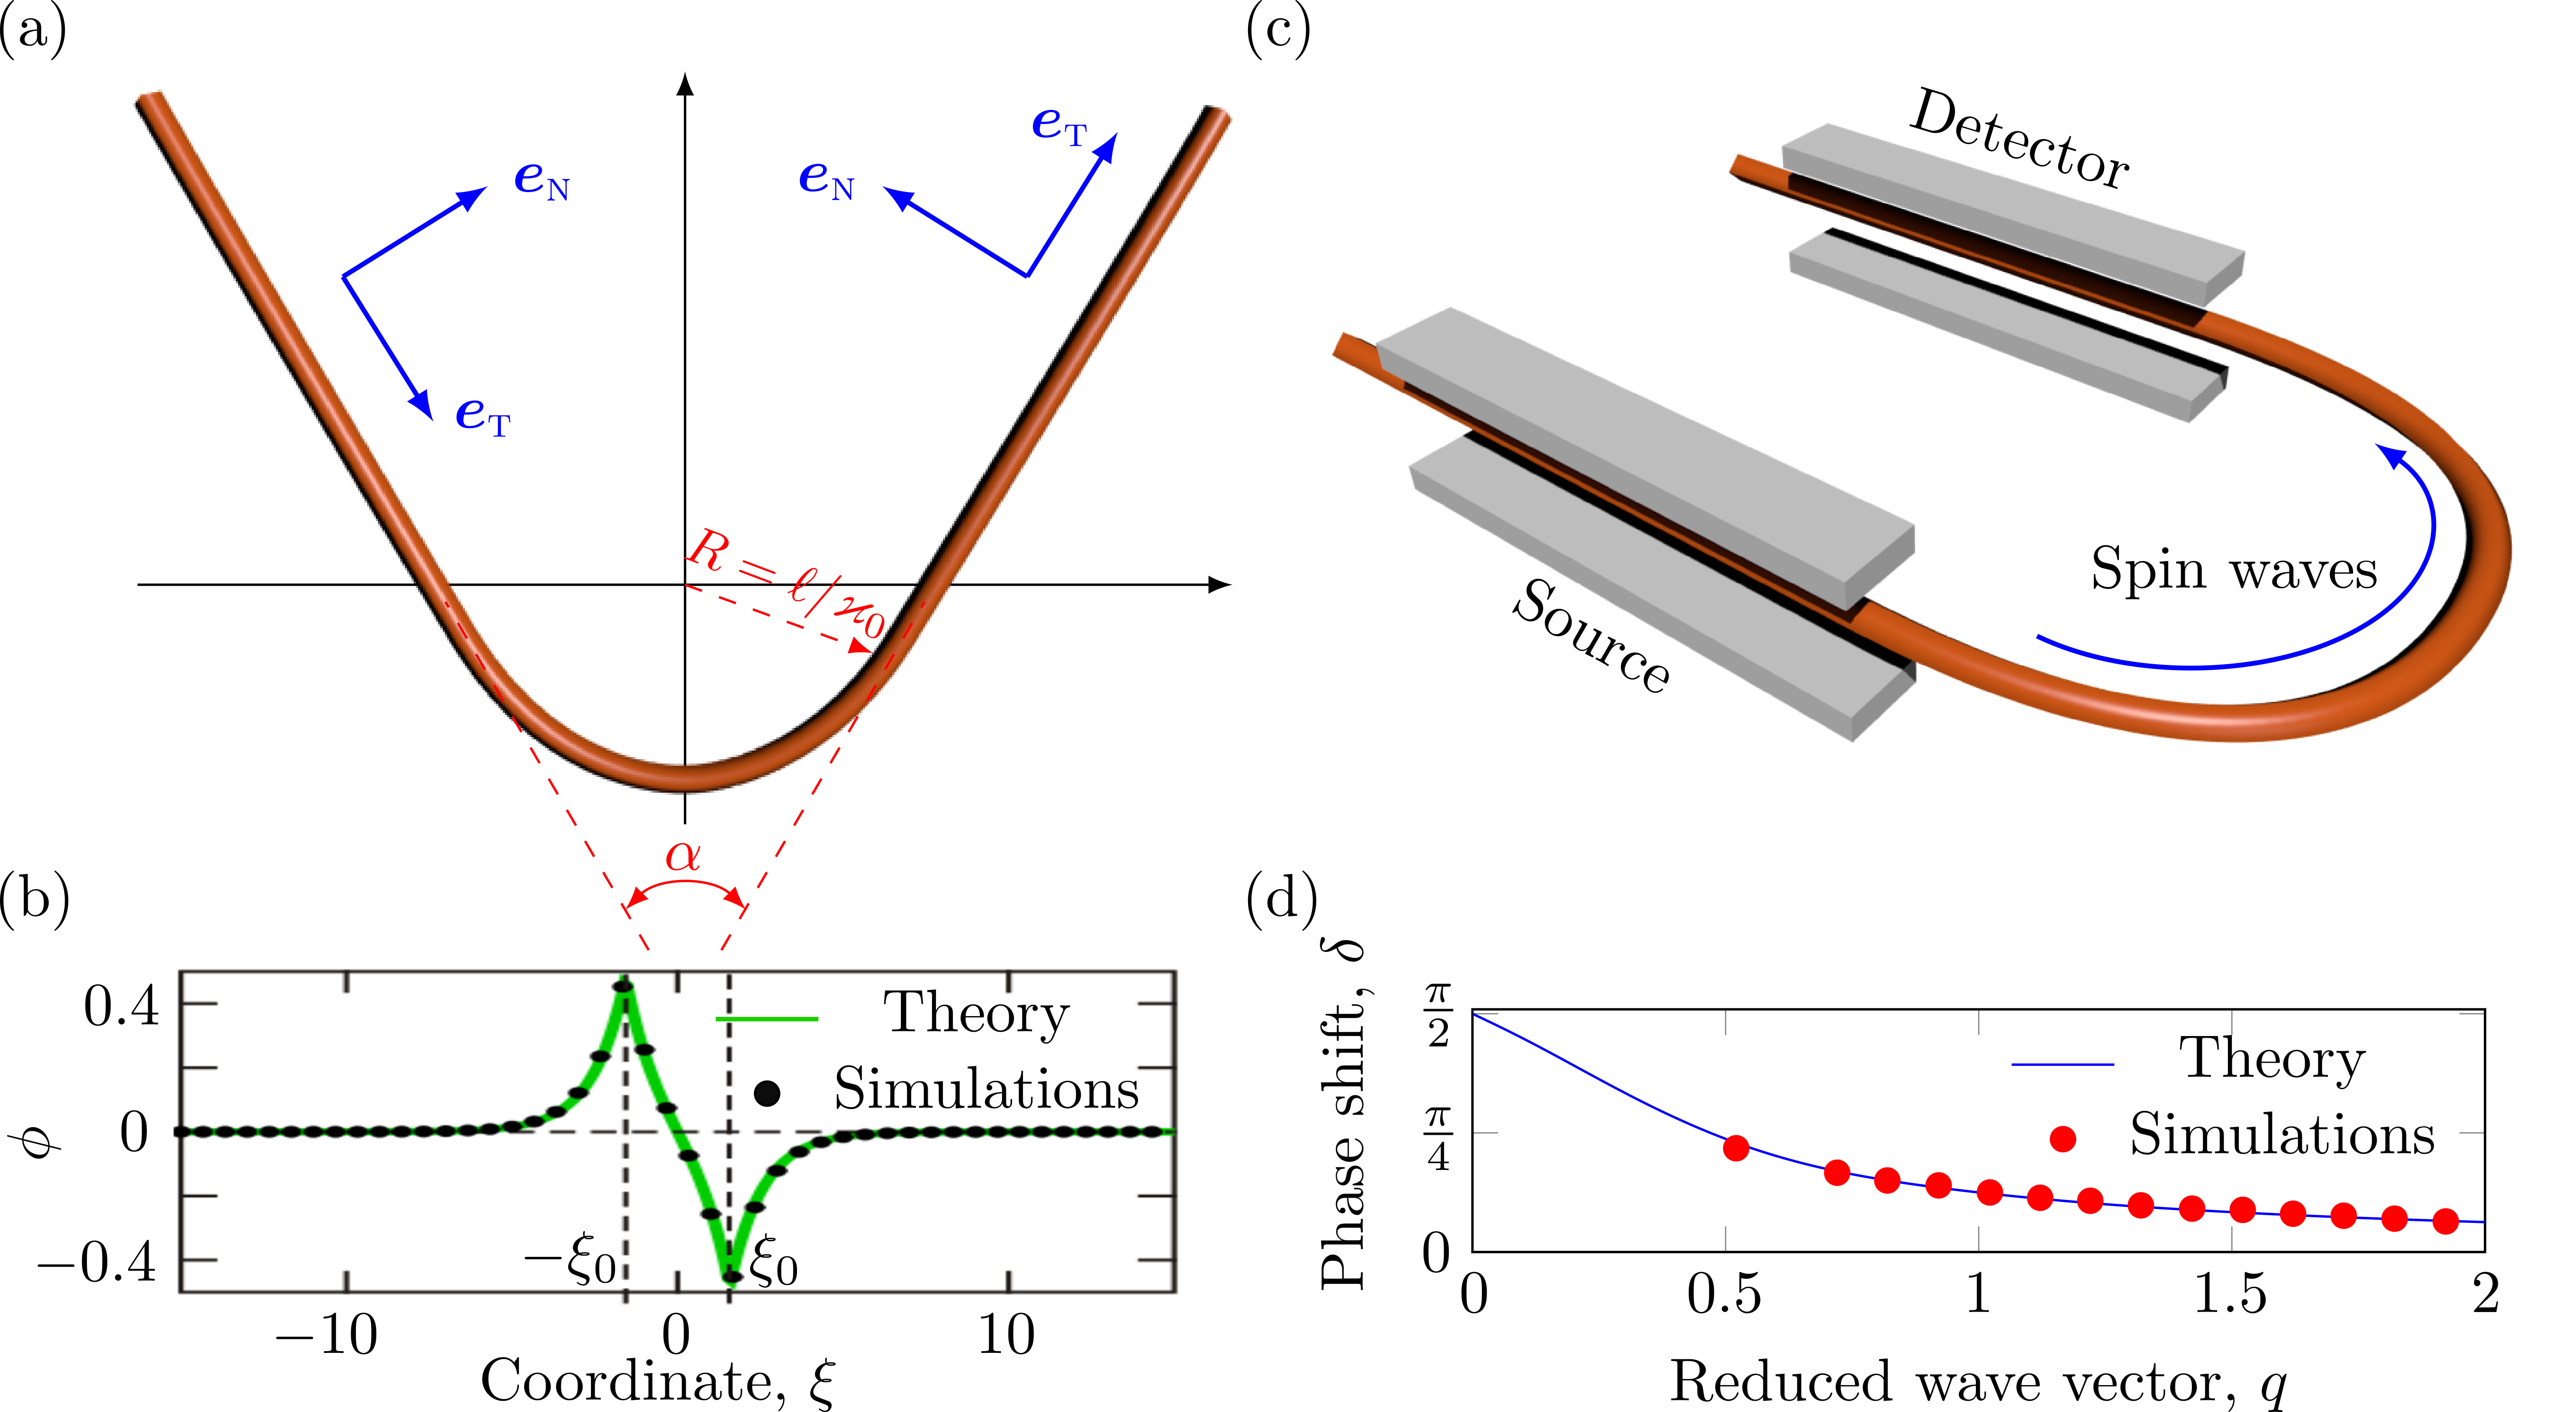
\includegraphics[width=1.0\linewidth]{fig_circular_segment}
	\end{center}
	\caption{
		\textbf{Wire with box-functional curvature:}
		(a) Curve with a box-function curvature with $R$ being the bending radius and $\alpha$ being the angle of expansion. 
		(b) Equilibrium magnetization state for the wire with the box curvature for	$\varkappa_0= 1$.
		(c) Schematic of bended ferromagnet wire. The spin wave is generated by an alternating field inside the ``Source'' region and propagates through the bend to  the detector. The phase of the transmitted wave is compared with the phase expected for the straight wire. 
		(d) Phase shift of the transmitted spin wave according to the \eqref{eq:Levinson} compared with spin-lattice simulations. Adapted with permission from~\cite{Gaididei18a}.}
	\label{fig:Circular_segment_1}
\end{figure}
%==================================================================/

The equilibrium state of the system corresponds to the minimum of the energy functional \eqref{eq:energy_angular}: the ground magnetization distribution for the considered wire is also planar and lies in the osculating (TN) plane. Thus, the equilibrium magnetic state has the form 
\begin{subequations} \label{eq:Theta-Phi-statics}
	\begin{equation} \label{eq:gs}
	\theta_0 = \frac{\pi}{2},\quad \phi_0 = \phi(\xi),
	\end{equation}
where the corresponding azimuthal magnetization angle $\phi$ is described by the driven pendulum equation~\cite{Gaididei18a}:
	\begin{equation} \label{eq:LL-statics-phi}
	\phi '' - \sin\phi  \cos\phi  = - \varkappa'.
	\end{equation}
\end{subequations}
In the limiting case of a smoothly curved wire with localized curvature $|\varkappa_0| \ll 1$, the ground state has a form of two hooks in the points of curvature step with exponential tails~\cite{Gaididei18a}, see Fig.~\ref{fig:Circular_segment_1}(b),
\begin{equation} \label{eq:boxcar-gs-linear}
\phi_0 =
\begin{cases}
-\varkappa_0 \, e^{-\xi_0} \, \sinh(\xi), & \text{when $|\xi|\leq \xi_0$},\\
-\varkappa_0 \, \text{sgn}(\xi) \, e^{-|\xi|} \, \sinh(\xi), &\text{when $|\xi|> \xi_0$}.
\end{cases}
\end{equation}
The maximal deviation of $\phi_0$ from the tangential direction takes place in points of junction of circular segment and straight wires, this is because of the curvature jump.


\subsubsection{Magnon eigenmodes and phase shift} \label{sec:box_curvature_eigenmodes}

To analyze magnon modes, it is instructive to consider the small deviations of the magnetization vector on the background of the static solution~\eqref{eq:Theta-Phi-statics}. We rewrite the linearized equations of motion \eqref{eq:ring_magnons} with complex scalar function $\psi=(\theta-\theta_0) + i \left(\phi-\phi_0\right)$  in the form of a generalized Schr\"odinger equation~\cite{Sheka04,Ivanov05b,Gaididei18a}
\begin{equation} \label{eq:Schroedinger}
-i \,\dot{\psi} = \mathcal{H} \, \psi + W \, \psi^\star, \qquad \mathcal{H} = -\partial_\xi^2 +1+U.
\end{equation}
Here, the star operator means the complex conjugation, and the geometry-induced potentials have the following form~\cite{Gaididei18a}
\begin{equation} \label{eq:V-n-W}
\begin{split}
U(\xi) &= -\frac{1}{2}\left[3\sin^2\phi_0  + \left(\phi_0 ' + \varkappa\right)^2\right],\\
W(\xi) &= \frac{1}{2}\left[\sin^2\phi_0  - \left(\phi_0 ' + \varkappa\right)^2\right].
\end{split}
\end{equation}
In the case of localized box-function curvature profile, the effective potentials are~\cite{Gaididei18a} 
\begin{equation} \label{eq:V-n-W-as}
U(\xi) \approx W(\xi) \approx
\begin{cases}
-\varkappa^2(\xi)/2, & \text{when $|\xi|\leq \xi_0$},\\
0, &\text{when $|\xi|> \xi_0$}.
\end{cases}
\end{equation}
Thus, the scattering problem of magnons by the localized bending region becomes equivalent to the scattering problem of a quantum particle inside the potential $U$. Analyzing the generalized Schr\"odinger equation~\eqref{eq:Schroedinger} allows to determine the appearance of local modes (bound states) inside the gap with the frequency~\cite{Gaididei18a} 
\begin{equation} \label{eq:omega-loc}
\Omega^{\text{loc}} = 1 - \frac{1}{16} \left[
\int_{-\infty}^{\infty} \varkappa^2(\xi)\mathrm{d}\xi\right]^2.
\end{equation}
These local modes are localized on a wire bend and have eigenfrequency below the ferromagnetic resonance $\omega_0$, see Table~\ref{tab:notation}. The interaction of the local modes with spin waves, propagating through the bend, results in a shift of the wave phase according to the quantum scattering theory and the Levinson theorem~\cite{Swan63}. Thus, the total phase shift $\delta_t(0)-\delta_t(\infty)$ is related to the number of bound states (i.e. local modes) $N^{\text{loc}}$ and half--bound states (i.e. half-local modes) $N^{\text{h.loc}}$~\cite{Ma06a}. 
In the 1D case the total phase shift reads~\cite{Dong00b}
\begin{equation} \label{eq:Levinson}
\frac{\delta_t(0)-\delta_t(\infty)}{\pi} = 
\begin{cases}
N_e^{\text{loc}} + \frac12 N_e^{\text{h.loc}} -\frac12, 	& \text{even parity},\\
N_o^{\text{loc}} + \frac12 N_o^{\text{h.loc}}, 			& \text{odd parity}.
\end{cases}
\end{equation}
The resulting scattering phase $\delta_t$ calculated for spin waves propagating through the one-dimensional nanowire with ring segment is plotted in Fig.~\ref{fig:Circular_segment_1}(d).

\subsection{Wire with periodical curvature distribution}

Here, we consider a flat anisotropic FM nanowire with a fixed cross-section of area $S$ and periodically repeated semicircles of curvature $\varkappa_0$~\cite{Korniienko19b}, i.e. meander geometry [see Fig.~\ref{fig:Geometries_n_curvatures}(c)]. The spatial distribution of the curvature of such a wire is the square-wave function $\varkappa(\xi) = (-1)^{\lfloor\xi/\xi_0\rfloor}\varkappa_0$ with period $2\xi_0$ and $\xi_0=\pi/\varkappa_0$ being the length of a semicircle. Here $\lfloor x \rfloor$ defines the integer part of $x$.

\subsubsection{Equilibrium state}

 Similarly to the case of the box-function curvature profile discussed in Sec.~\ref{sec:box_curvature_equilibrium}, here we also have a planar magnetization distribution within wires plane~\cite{Korniienko19b}. The ground state is described by Eqs.~\eqref{eq:Theta-Phi-statics} with azimuthal angle $\phi$ defined as
\begin{equation}\label{eq:phi_meander}
\phi_0 = (-1)^\lambda \text{am}\left[\frac{\xi-\xi_0\left(\lambda+1/2\right)}{k},ik\right],\quad \lambda=\lfloor \xi/\xi_0 \rfloor,\quad k=\frac{1}{\sqrt{\varkappa_0^2-\sin^2\varphi_0}},
\end{equation}
where $\varphi_0=|\phi\left(n\xi_0\right)|$ is maximal value of the function $\phi(\xi)$ [see Fig.~\ref{fig:meander}(b)], it is determined by the equation $2kF(\varphi_0,ik) = \xi_0$, where $F(x,y)$ is elliptic integral of the first kind~\cite{NIST10} and the modulus $k = k(\varphi_0)$ is defined in~\eqref{eq:phi_meander}. One should note that the curvature amplitude $\varkappa_0$ is the only parameter which controls the system. The maximal deviation $\varphi_0$ from the tangential direction takes place in points of junction of two semicircles, this is because of the curvature jump. Depending on the $\varkappa_0$ one obtains two different behaviors~\cite{Korniienko19b}: (i) In the limit case of small curvature $\varkappa_0\ll1$ and due to the easy-tangential anisotropy the wire is magnetized practically tangentially except the junction points, where the magnetization demonstrates the small deviations of amplitude $\varphi_0\approx\varkappa_0$. (ii) In the opposite case of large curvature $\varkappa_0\gg1$ exchange interaction is dominating and results in quasi uniform magnetization aligned with $x$-axis with $\varphi_0\lesssim\pi/2$.

%==================================================================\
\begin{figure}[t]
	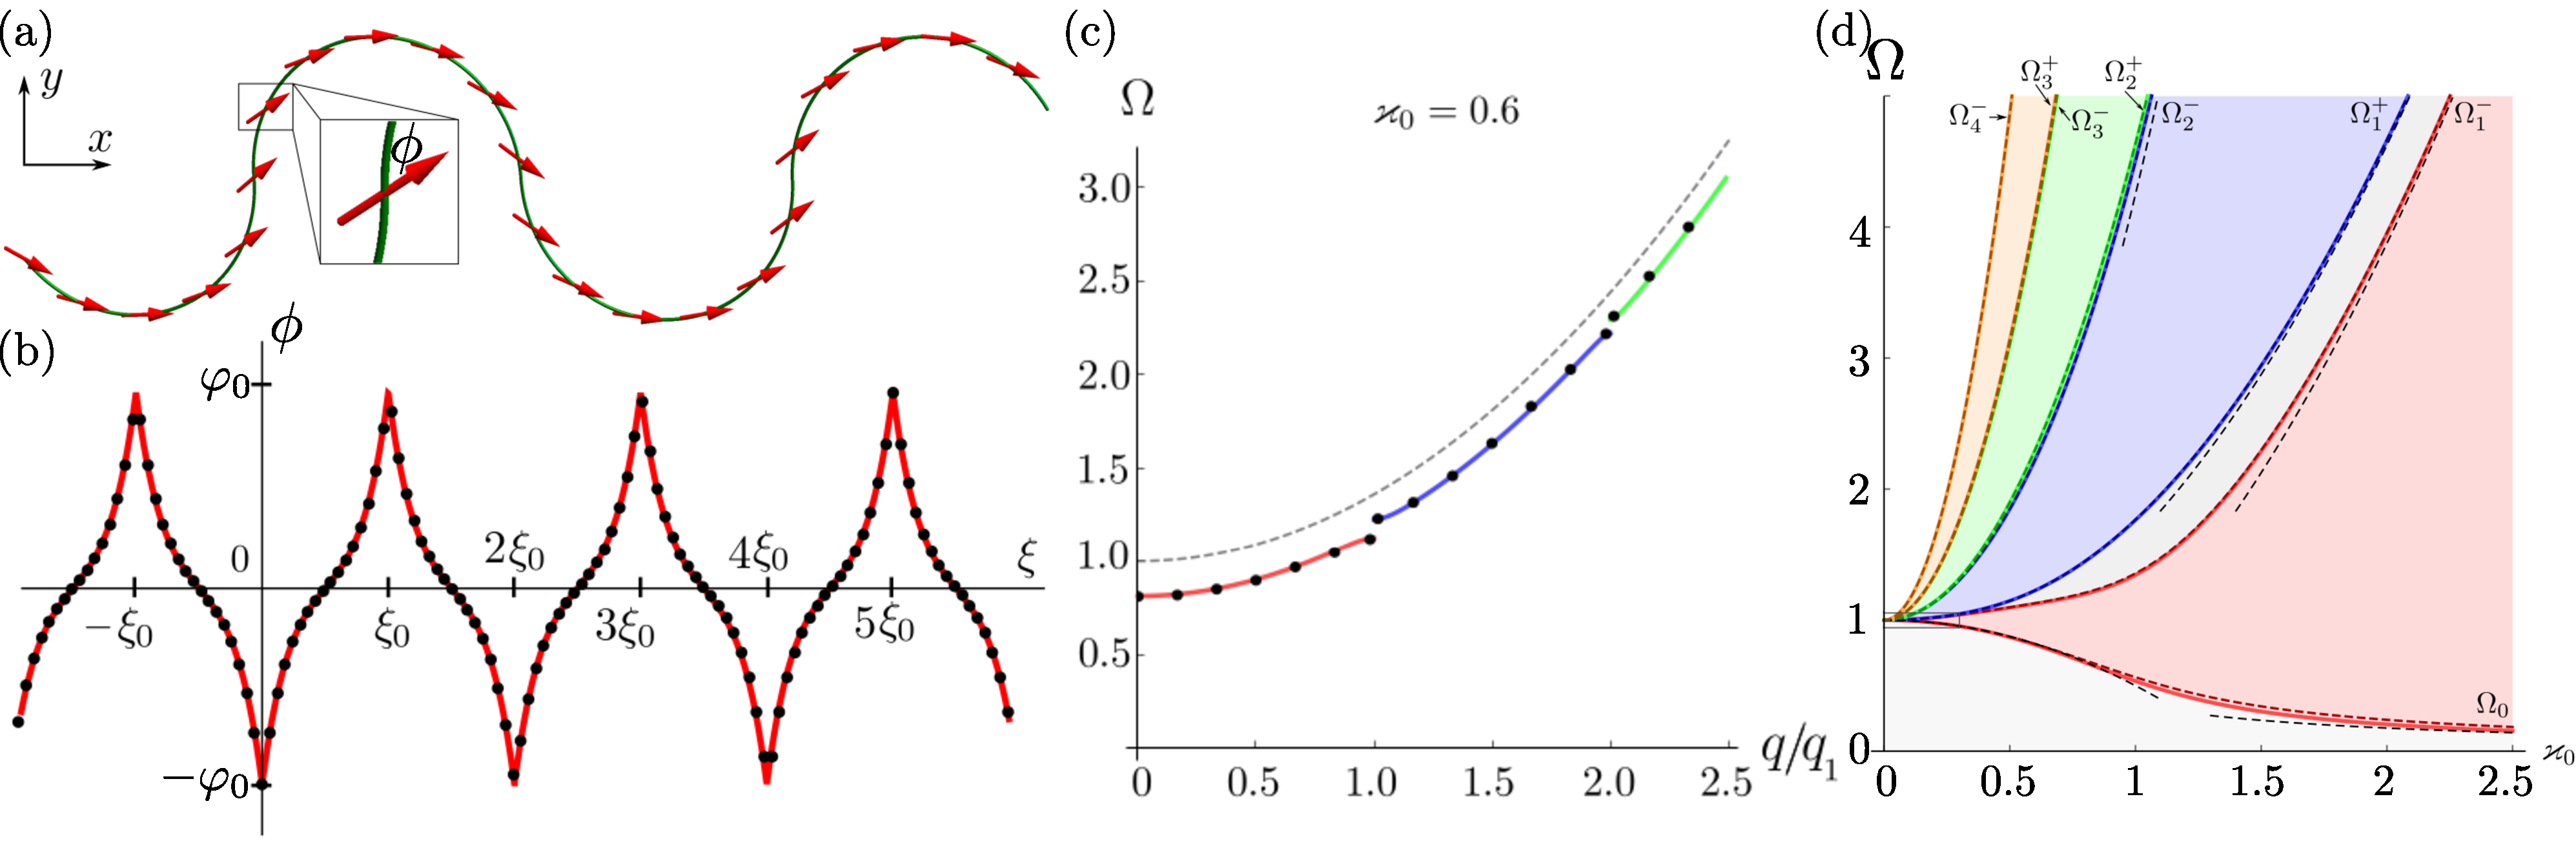
\includegraphics[width=\textwidth]{fig_meander}
	\caption{\label{fig:meander}%
		\textbf{Meander shaped wire:} (a) Spatial distribution of magnetization (red arrows) along the wires with the shape of meander; the inclination angle $\phi$ is shown in insets. (b) Azimuthal angle $\phi$ as function of arc length for meander shaped wire with $\varkappa_0=0.6$: line -- analytical solution, dots -- results of numerical simulations. (c) Dispersion relation for meander nanowire with  $\varkappa_0=0.6$. The dashed line shows the dispersion relation of a straight wire ($\varkappa_0=0$). The wavevector is normalized by $q_1=\varkappa_0$ corresponding to the edge of the first Brillouin zone. (d) The band structure as function of $\varkappa_0$. The first four bands of the magnon conductance are shown by different colours and gaps are shown by grey shading. Solid and dashed thick lines correspond to the exact numerical solution and to the approximations~\eqref{eq:band_gaps_meander}, respectively. Adapted with permission from~\cite{Korniienko19b}.}
\end{figure}
%==================================================================/

\subsubsection{Band structure}

The linear dynamics of magnetization in the meander shaped nanowire can be described by the generalized Schr\"odinger equation~\eqref{eq:Schroedinger} with geometry-induced potentials
\begin{equation} \label{eq:V-n-W_meander}
W(\xi) = \frac{\varkappa_0}{k}\sqrt{1+k^2\sin^2\phi_0}-\frac{1}{2}\left(\frac{1}{k^2}+\varkappa^2_0\right),\quad U(\xi) = W-2\sin^2\phi_0,
\end{equation}
where $\phi_0$ is determined in~\eqref{eq:phi_meander}. One should note that potentials $V(\xi)=V(\xi+\xi_0)$ and $W(\xi)=W(\xi+\xi_0)$ have twice as small period as $\phi_0(\xi)$ has, this is because the dependence on $\xi$ is reduced to the dependence on $\sin^2\phi_0(\xi)$ in~\eqref{eq:V-n-W_meander}. The periodic potential in a quantum mechanical Schr\"odinger equation always produces the band structure. Therefore, one can consider the the meander shaped wire as an magnonic crystal. In contrast to the straight wire, the dispersion relation for a given curvature $\varkappa_0>0$ demonstrates the frequency reduction and appearance of the band structure, see Fig.~\ref{fig:meander}(c). The band gap edges can be estimated as~\cite{Korniienko19b}
\begin{equation}
\Omega^{\pm}_\nu\approx\sqrt{\left(q^2_\nu+1+\mathcal{U}_0\mp \mathcal{U}_\nu\right)^2-\left(\mathcal{W}_0\mp \mathcal{W}_\nu\right)^2}, \quad \nu\in\mathbb{N}.
\end{equation}
Here $\Omega^{+}_\nu$ and $\Omega^{-}_\nu$ correspond to the top and bottom edges of the $\nu$-th gap, respectively, $q_\nu = \nu\varkappa_0$ is a wavevector which corresponds to the edge of the $\nu$-th Brillouin zone, coefficients $\mathcal{U}_n$ and $\mathcal{W}_n$ denote Fourier components of the effective potentials $U$ and $W$, respectively. The size of the main gap $\Omega_0$ can be approximated as~\cite{Korniienko19b}
\begin{equation}\label{eq:band_gaps_meander}
\Omega_0\approx\sqrt{\left(1+\mathcal{U}_0\right)^2-\mathcal{W}_0^2}
\end{equation}
with Fourier coefficients
\begin{equation}
	\mathcal{U}_0 \approx -\frac{\varkappa_0^2}{2}\tanh^2\frac{\xi_0}{2}, \quad \mathcal{W}_0 \approx -\frac{\varkappa_0^2}{2}\left[1+\frac{1}{\cosh^2\frac{\xi_0}{2}} - \frac{4}{\xi^2}\tanh\frac{\xi_0}{2}\right].
\end{equation}
For the case of the small curvature amplitude $\varkappa_0\ll 1$ one obtains $\Omega_0\approx1 - \varkappa_0^2/2$, while for the large curvature amplitude $\varkappa_0\gg1$ we have $\Omega_0\approx 1/\left(2\sqrt{2}\varkappa_0\right)$, see Fig.~\ref{fig:meander}(d).

%\subsection{Spiral nanowire with $\kappa' =$ const} \label{subsec:Spiral_wire}

%\subsection{Nanowire with localized curvature gradient} \label{subsec:Parabolic_wire}

Magnetic properties of ferromagnetic elements at the nanoscale are governed not only by the intrinsic material properties, but also by geometries of elements. This dependence manifests itself during the motion of magnetization textures and their magnetic responses to the external influences. Thus, the appropriately engineered geometry of magnetic elements can introduce additional local energy minima in a small magnetic structures, which can for instance be set to a multidomain state due to the magnetostatic interaction that favors magnetization alignment along the element edges. These can result in a reproducible and controlled formation of domain walls in magnetic curvilinear geometries. The behavior of domain walls in planar curvilinear magnetic nanowires is a topic of great technological interest due to their perspective application in modern memory~\cite{Hayashi07,Parkin08} and logic devices~\cite{Allwood02,Allwood04,Allwood05,Hayashi08}. The suitability of domain walls for these application originate from their topological stability and particle-like properties, which allow them to be assigned as an information carrier in a similar manner to charge signals in conventional microelectronic systems~\cite{Klaui08,Jiang11,Negoita12}. The modification of dynamics and static properties of a domain wall due to the wire curvature is of high importance for the application, due to the influence of localized curvilinear defects on the appearance of pinning potential for domain walls~\cite{Lewis09,Glathe12,Burn14}. This means that changes in local geometrical shapes engineer the energetic landscape, that can be utilized for the precise positioning of domain walls. 

\subsubsection{Domain walls in parabolic nanowire} \label{subsubsec:Parabola_theory}

To demonstrate the influence of the exchange-induced chiral effects on magnetic domain walls in nanowire with localized curvature, we will consider here the case of parabolic wire geometry:
\begin{equation} \label{eq:parabola_wire}
	\vec{\gamma} = x \, \hat{\vec{x}} + \dfrac{\kappa_0 \, x^2}{2} \, \hat{\vec{y}},
\end{equation}
which is the mathematically simplest possible curve with well-defined geometry and curvature distribution:
\begin{equation}
	\kappa = \dfrac{\kappa_0}{(1+\kappa^2_0 \, x^2)^{3/2}}.
\end{equation}  

For the further analysis it is convenient to rewrite the total micromagnetic energy~\eqref{eq:total_energy} in the normalized form, $\mathcal{E} = E/4 \, \pi \, M_s^2$, by using the angular magnetic parameterization $\vec{m} = \cos\theta \, \vec{e}_{\textrm{T}}+\sin\theta \, \cos\phi \, \vec{e}_{\textrm{N}} + \sin\theta \, \sin \phi \, \vec{e}_{\textsc{B}}$, 
\begin{equation}\label{eq:Parabola_total_energy}
	\begin{split}
		\mathcal{E} &= S \, \int^{+ \infty}_{-\infty}\mathrm{d}\vec{s} \, \left[\ell^2 \, (\theta' + \kappa \, \cos \phi)^2 + \ell^2 (\phi' \, \sin \theta  - \kappa \, \cos \theta \, \sin \phi)^2 -k_t \, \cos^2 \theta \right],
	\end{split}
\end{equation}
where $S$ is the area of the wire cross section, $\ell = \sqrt{A/(4 \, \pi \, M^2_s)}$ is the exchange length and $k_t = K/(4 \, \pi \, M^2_s) + 1/4$ is the dimensionless anisotropy constant. The equilibrium magnetic state for \eqref{eq:Parabola_total_energy} could be determined by means of the energy minimization technique, which results in a planar solution with $\phi = \phi_0 = 0, \, \pi$ and $\theta$ determined by an inhomogeneous Sine-Gordon equation 
\begin{equation} \label{eq:Parabola_theta_equation}
	\ell^2_m \, \theta'' - \sin \theta \, \cos \theta = - \ell^2_m \, \kappa' \, \cos \phi_0,
\end{equation}
where $\ell_m = \ell/\sqrt{k_t}$ is the magnetic length.

For the case $\kappa' = 0$, which takes place in rectilinear and circular wires, the Eq.~\eqref{eq:Parabola_theta_equation} has a well known domain wall solution $\cos \theta = - p \, \tanh[(s-q)/\Delta]$, where $p$ is the domain wall polarity: $p=1$ for head-to-head and $p=-1$ for tail-to-tail domain walls, respectively. Here $q$ determines the domain wall position along the wire and $\Delta = \ell_m$ is the wall width. For the case $\kappa' \neq 0$ an additional driving force appears and the curvature-induced domain wall dynamics is expected. 

To analyze the domain wall properties, it is instructive to use a collective variable approach~\cite{Slonczewski72,Thiele73} based on the simple $q$ -- $\Phi$ model~\cite{Slonczewski72,Malozemoff79} 
\begin{equation} \label{eq:q-phi_model}
	\cos \theta = - p \, \tanh \left[ \dfrac{s-q(t)}{\Delta} \right], \qquad \phi = \Phi(t).
\end{equation}
The domain wall position $q$ and phase $\Phi$, which determines orientation of the transversal magnetization component, make a cononically conjugated pair of collective variables. Substituting the model Ansatz \eqref{eq:q-phi_model} to \eqref{eq:Parabola_total_energy} one obtains the resulting energy of the domain wall~\cite{Yershov15b}
\begin{equation} \label{eq:DW_total_energy}
	\dfrac{\mathcal{E}}{2 \, S} = \left( \dfrac{\ell^2}{\Delta} + k_t \, \Delta \right) + \pi \, p \, \ell^2 \, \kappa(q) \, \cos\Phi - \ell^2 \, \kappa^2(q) \, \Delta \, \sin^2 \Phi,
\end{equation}
where the condition $\kappa \, \Delta \ll 1$ was applied during the integration. The first term in \eqref{eq:DW_total_energy} corresponds to the interplay between exchange interaction and magnetic anisotropy, which determines the domain wall width similar to the case of a rectilinear wire. The second and the third terms are curvature-induced exchange-driven effective DMI-like and anisotropy-like terms~\cite{Yershov15b,Sheka15}. Minimization of the total energy of the domain wall \eqref{eq:DW_total_energy} with respect ot collective variables $q$ and $\Phi$ results in the following equilibrium values $q_0$ and $\Phi_0$:
\begin{equation} \label{eq:qPhi_equilibrium}
	\kappa'(q_0) = 0, \qquad \cos \Phi_0 = -p.
\end{equation} 
The exchange-driven effective DMI leads to the reshaping of the domain wall total energy \eqref{eq:DW_total_energy} in a way of appearance additional potentials corresponding to the type of domain walls: (i) In the case of two transversal domain walls with $p=+1$, $\Phi=\pi$ (head-to-head) and with $p=-1$, $\Phi=0$ (tail-to-tail) the curvature-induced DMI form a potential well at the apex region, see Fig.~\ref{fig:Parabola_n_straight_DWs}(a). (ii) In the case of two other possible configuration of transversal domain walls with $p=+1$, $\Phi=0$ (head-to-head) and with $p=-1$, $\Phi=\pi$ (tail-to-tail), there is a potential wall, see Fig.~\ref{fig:Parabola_n_straight_DWs}(b).  This is in contrast to a straight stripe system, where all four possible types of transversal DWs are energetically equal and stable in a sense of neutral equilibria in the $q$ -- $\Phi$ model framework, see Fig.~\ref{fig:Parabola_n_straight_DWs}(c).

%==================================================================\
%\begin{figure}[t]
%	\center{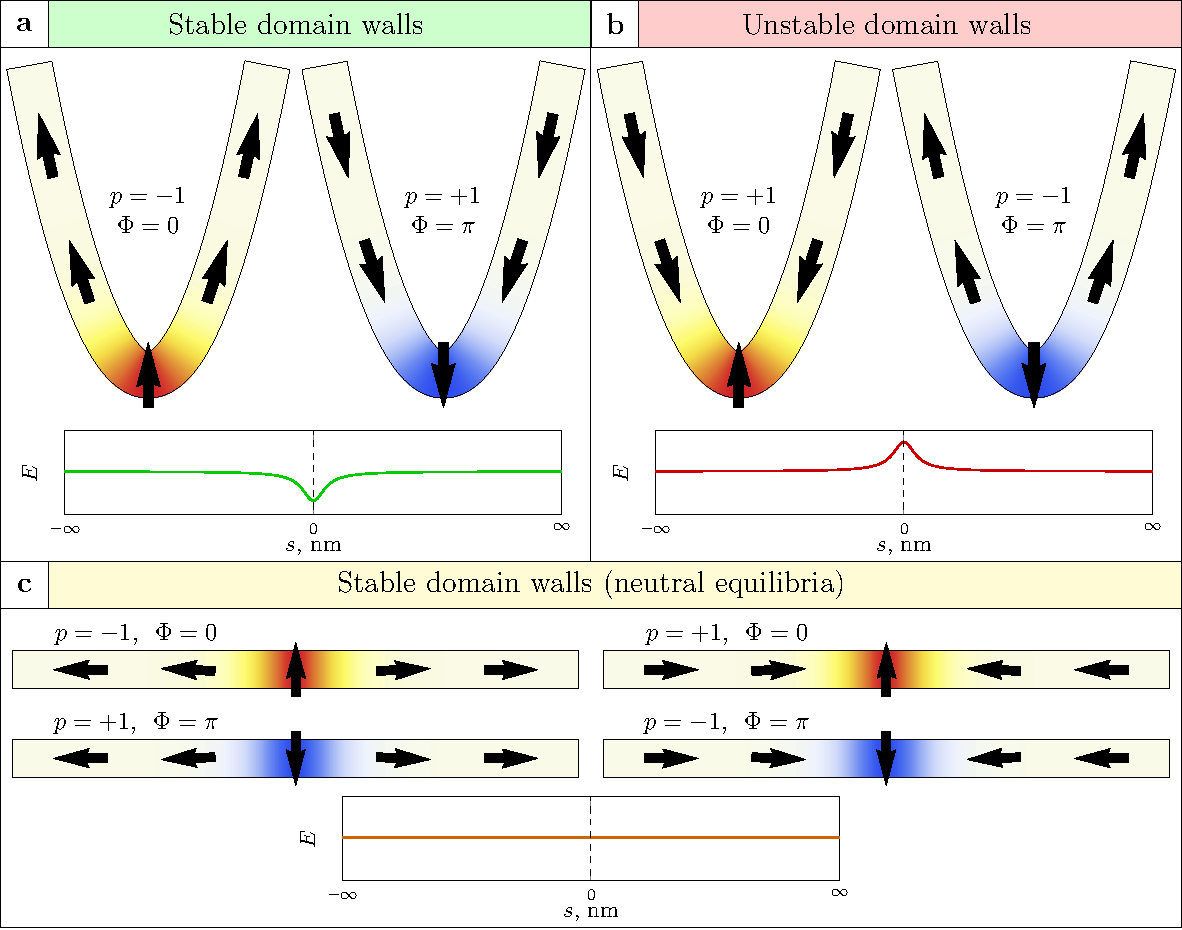
\includegraphics[width=0.9\linewidth]{Parabola_n_straight_stripe_sketch_SupplMat_1}}
%	\caption{\textbf{Curvature-induced asymmetrical stability of transversal DWs and their comparison with similar DWs in straight stripes.} \textbf{(a)},~Stable tail-to-tail and head-to-head DWs and their energy landscape on DWs position along the parabolic stripe. The energy landscape is calculated by means of the $q$ -- $\Phi$ model. The potential well at the apex region appears due to the influence of the curvature-induced DMI. \textbf{(b)},~Unstable head-to-head and tail-to-tail transversal DWs in a parabolic stripe and corresponding to them potential wall. \textbf{(c)},~Transversal DWs in a straight stripe, with their neutral stability within the framework of the $q$ -- $\Phi$ model. Adapted with permission from~\cite{Volkov19c}.}
%	\label{fig:Parabola_n_straight_DWs}
%\end{figure}
%==================================================================/

As it follows from~\eqref{eq:q-phi_model}, the equilibrium value of the domain wall width $\delta_0 = \ell_m$ is the same as for a straight wire. However, if the wall is not in the equilibrium position and the collective variables $(q,\Phi)$ deviate from the equilibrium \eqref{eq:qPhi_equilibrium}, the domain wall width is modified as follows~\cite{Yershov15b}
\begin{equation}
	\Delta(q, \, \Phi) = \dfrac{\ell}{\sqrt{k_t - k_b \, \sin^2 \Phi}},
\end{equation}
where $k_b = \ell^2 \, \kappa^2(q)$ is a coefficient of the curvature-induced effective easy-binormal anisotropy. 



\subsubsection{Domain walls dynamics} \label{subsubsec:Parabola_dynamics}

To analyze domain wall dynamics in the parabolic nanowire it is convenient to consider the equations of motions for the collective variables $q$ -- $\Phi$~\cite{Yershov15b}, as follows
\begin{equation} \label{eq:qPhi_dynamics}
	\dot{q} = \dfrac{\omega_0}{2 \, S} \, \dfrac{\partial \mathcal{E}}{\partial \Phi} + \alpha \, \Delta \, \dot{\Phi}, \qquad \dot{\Phi} = - \dfrac{\omega_0}{2 \, S} \, \dfrac{\partial \mathcal{E}}{\partial q} - \dfrac{\alpha}{\Delta} \, \dot{q}.
\end{equation}

The domain wall motion in the vicinity of the equilibrium position could be described by means of small deviations $q(t) = q_0 + \tilde{q}(t)$ and $\Phi(t) = \Phi_0 + \tilde{\Phi}(t)$. In the limit case of $\kappa \Delta_0 \rightarrow 0$ the equation of motion \eqref{eq:qPhi_dynamics} linearized with respect to the deviations read~\cite{Yershov15b}
\begin{equation} \label{eq:qPhi_linear_dynamics}
	(1+\alpha^2) \, \begin{Vmatrix*} \dot{\tilde{q}} \\ \dot{\tilde{\Phi}} \end{Vmatrix*} \approx \omega_0 \, \ell^2 \, \pi \, \begin{Vmatrix*} \, 0 \qquad	& \, \, \, \kappa(q_0) \, \\
	\, \kappa''(q_0) \qquad	& \, \, \, - \alpha \, \frac{\kappa(q_0)}{\Delta_0} \, \end{Vmatrix*} \cdot \begin{Vmatrix*} \tilde{q} \\ \tilde{\Phi} \end{Vmatrix*}.
\end{equation}
For the case of small $\alpha$ the solution of \eqref{eq:qPhi_linear_dynamics} results in harmonic decaying oscillations $\tilde{q} \propto \sin(\Omega \, t + \delta_0) \, e^{-\eta \, t}$ and $\tilde{\Phi} \propto \cos(\Omega \, t + \delta_0) \, e^{-\eta \, t}$ with frequency~\cite{Yershov15b}
\begin{equation} \label{eq:Omega_1}
	\Omega \approx \omega_0 \, \ell^2 \, \pi \, \sqrt{\kappa(q_0) \, |\kappa''(q_0)|}
\end{equation}
and modified effective friction 
\begin{equation} \label{eq:eta_1}
	\eta \approx \alpha \, \omega_0 \, \dfrac{\pi}{2} \, \dfrac{\ell^2 \, \kappa(q_0)}{\Delta_0}.
\end{equation}
The phase $\delta_0$ is determined by the initial conditions. In the case of parabolic wire the eigenfrequency \eqref{eq:Omega_1} and effective friction \eqref{eq:eta_1} reads~\cite{Yershov15b}
\begin{equation} \label{eq:Omega_eta_2}
	\Omega \approx \omega_0 \, \sqrt{3} \, \pi \, (\kappa_0 \, \ell)^2, \qquad \eta \approx \alpha \, \omega_0 \, \ell \, \kappa_0 \, \dfrac{\pi}{4}.
\end{equation}
These results were verified by means of full-scale and one-dimensional micromagnetic simulations for various apex curvatures, see Fig.~\ref{fig:DW_dynamics_parabola}.

%==================================================================\
\begin{figure}
	\center{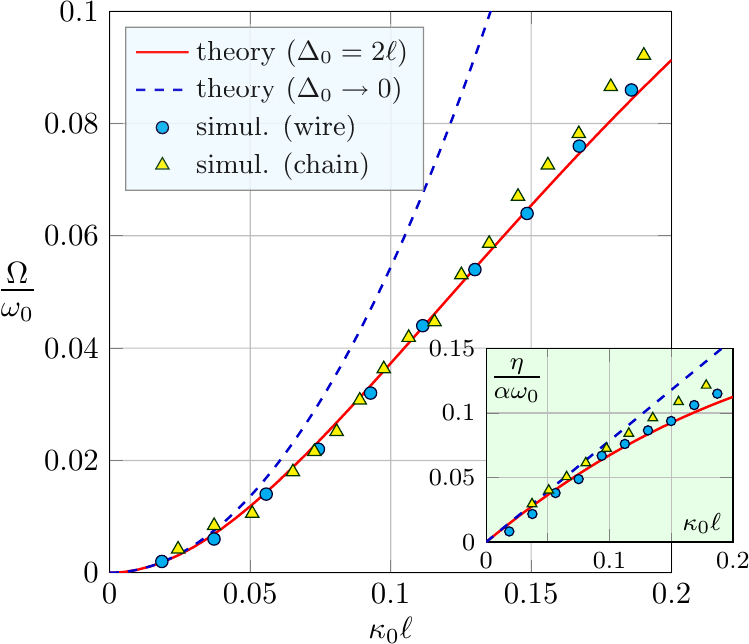
\includegraphics[width=0.5\linewidth]{DW_parabola_dynamics.png}}
	\caption{\textbf{Eigenfrequency and effective friction of the domain wall oscillations in vicinity of the equilibrium.} Solid and dashed lines correspond to the analytical predictions~\eqref{eq:Omega_eta_2}. Markers show the results of numerical simulations for nanowires (disks) and discrete chains of magnetic moments (triangles). 
	Adapted with permission from~\cite{Yershov15b}.}
	\label{fig:DW_dynamics_parabola}
\end{figure}
%==================================================================/


